
\chapter{无字证明}
\label{chap:proofs-without-words}

\epigraph{一图胜千言,一表胜万卷。}{}

无字证明(Proof without Words)是指仅用图像而无需文字解释就能不证自明的数学命题。然而无字证明并不是严格的数学证明,只是帮助直观理解。

\section{代数}
\label{sec:pww-algebra}

\begin{example}
  前$n$个奇数的和等于$n^2$,即
  \begin{align}
    \underbrace{1 + 3 + 5 + \cdots + (2n-1)}_{n\text{个}} = n^2
  \end{align}
\end{example}

\begin{center}
  \begin{tikzpicture}[scale=0.6]
    \begin{scope}[shift={(0,0)}]
      \foreach \r/\f in{1/white,2/red!30,3/white,4/blue!30,5/white,6/violet!30}{
        \draw[fill=\f](-\r,-\r) rectangle(\r-1,1-\r);
        \draw(-\r,-\r)grid(\r-1,1-\r);
        \draw[pattern=north east lines, pattern color=black](-1,-\r) rectangle(0,1-\r);
      }    
    \end{scope}
    \begin{scope}[shift={(7,0)}]
      \draw[|<->|](0,0)--(0,-6) node[midway,fill=white]{$n$层};
    \end{scope}
    \begin{scope}[shift={(9,0)}]
      \foreach \r/\f in{1/white,2/red!30,3/white,4/blue!30,5/white,6/violet!30}{
        \draw[fill=\f](0,-\r) rectangle(\r,1-\r);
        \draw(0,-\r)grid(\r,1-\r);
        \draw[fill=\f](\r,0) rectangle(\r-1,-\r);
        \draw(\r,0) grid(\r-1,-\r);
        \draw[pattern=north east lines, pattern color=black](\r-1,1-\r) rectangle(\r,-\r);
      }
    \end{scope}
  \end{tikzpicture}
\end{center}

\begin{example}
  前$n$个数的和是$\dfrac{(n+1)}{2}$,即
  \begin{align}
    1+2+3+\cdots+n=\frac{n(n+1)}{2}
  \end{align}
\end{example}
\begin{center}
  \begin{tikzpicture}[scale=0.6]
    \begin{scope}[shift={(0,0)}]
      \foreach \r/\f in{1/white,2/red!30,3/white,4/blue!30,5/white,6/violet!30}{
        \draw[fill=\f](0,1-\r) rectangle(\r, -\r);
        \draw(0,1-\r) grid(\r, -\r);
      }    
    \end{scope}
    \begin{scope}[shift={(8,0)}]
      \draw[|<->|](0,0)--(0,-6) node[midway,fill=white]{$n$层};
    \end{scope}
    \begin{scope}[shift={(10,0)}]
      \foreach \r/\f in{1/white,2/red!30,3/white,4/blue!30,5/white,6/violet!30}{
        \draw[fill=\f](0,1-\r) rectangle(\r, -\r);
        \draw(0,1-\r) grid(\r, -\r);
      }
      \foreach \r/\f in{1/violet!30,2/white,3/blue!30,4/white,5/red!30,6/white}{
        \draw[fill=\f](\r,1-\r) rectangle(7, -\r);
        \draw(\r,1-\r) grid(7, -\r);
      }
      \draw[very thick](1,0)--(1,-1)--(2,-1)--(2,-2)--(3,-2)--(3,-3)
                     --(4,-3)--(4,-4)--(5,-4)--(5,-5)--(6,-5)--(6,-6);
      \draw[|<->|](0,-7)--(7,-7) node[midway,fill=white]{$n+1$};      
    \end{scope}
  \end{tikzpicture}
\end{center}

\begin{example}
  \begin{align*}
    1+2+3+\cdots+(n-1)=\binom n2
  \end{align*}
  \begin{center}
    \begin{tikzpicture}[scale=1.0]
      \begin{scope}[shift={(0,0)}]
        \foreach \x/\y in {
          0/0,
          -.6/-1,.6/-1,
          -1.2/-2,0/-2,1.2/-2,
          -1.8/-3,-.6/-3,.6/-3,1.8/-3,
          -2.4/-4,-1.2/-4,0/-4,1.2/-4,2.4/-4,
          -3.0/-5,-1.8/-5,-.6/-5,.6/-5,1.8/-5,3.0/-5
          }{
            \draw[fill=yellow!30](\x,\y)circle(.5);
          }
          \foreach \x/\y in {
            -3.6/-6,-2.4/-6,-1.2/-6,0/-6,1.2/-6,2.4/-6,3.6/-6
          }{
            \draw[pattern=north west lines](\x,\y)circle(.5);
          }
          \draw[->](.6,-3)--(-1.2,-6);
          \draw[->](.6,-3)--(2.4,-6);
      \end{scope}
    \end{tikzpicture}
  \end{center}

  如图,在$7$个带阴影的圆中选$2$个,每种选法与其上某个圆圈一一对应,即三个圆圆心组成一个等腰三角形。
\end{example}

\pagebreak
\newcommand{\fixedcirclenode}[3]{\draw #1 circle(#2) node {#3};}
\begin{example}
  \begin{align*}
    1^2+2^2+3^2+\cdots=\frac{n(n+1)(2n+1)}6
  \end{align*}
  \centering
  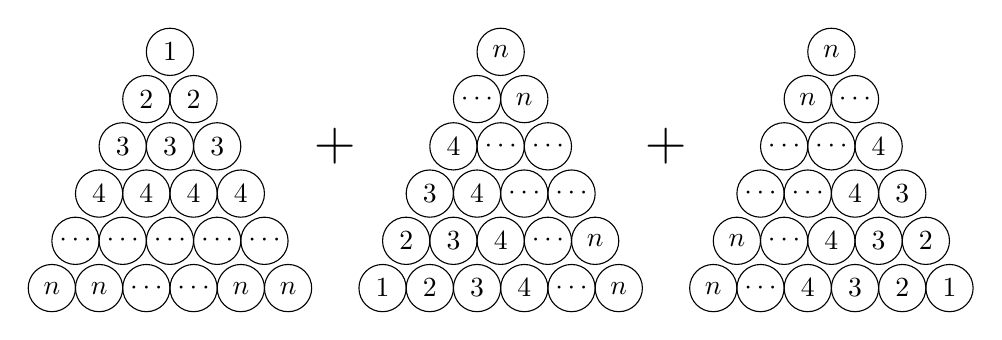
\begin{tikzpicture}[scale=.6]
    \begin{scope}[shift={(0,0)}]
      \fixedcirclenode{(0,0)}{.5}{1};
      \fixedcirclenode{(-.5,-1)}{.5}{2}; \fixedcirclenode{(.5,-1)}{.5}{2};
      \fixedcirclenode{(-1,-2)}{.5}{3};  \fixedcirclenode{(0,-2)}{.5}{3};  \fixedcirclenode{(1,-2)}{.5}{3}; 
      \fixedcirclenode{(-1.5,-3)}{.5}{4};  \fixedcirclenode{(-.5,-3)}{.5}{4};  \fixedcirclenode{(.5,-3)}{.5}{4}; \fixedcirclenode{(1.5,-3)}{.5}{4}; \fixedcirclenode{(-2,-4)}{.5}{$\cdots$};
      \fixedcirclenode{(-1,-4)}{.5}{$\cdots$};  \fixedcirclenode{(0,-4)}{.5}{$\cdots$}; \fixedcirclenode{(1,-4)}{.5}{$\cdots$}; \fixedcirclenode{(2,-4)}{.5}{$\cdots$}; 
      \fixedcirclenode{(-2.5,-5)}{.5}{$n$}; \fixedcirclenode{(-1.5,-5)}{.5}{$n$};  \fixedcirclenode{(-.5,-5)}{.5}{$\cdots$};  \fixedcirclenode{(.5,-5)}{.5}{$\cdots$}; \fixedcirclenode{(1.5,-5)}{.5}{$n$}; \fixedcirclenode{(2.5,-5)}{.5}{$n$}; 
    \end{scope}
    
    \begin{scope}[shift={(3.5,0)}]
      \node at (0,-2) {{\huge $+$}};
    \end{scope}

    \begin{scope}[shift={(7,0)}]
      \fixedcirclenode{(0,0)}{.5}{$n$};
      \fixedcirclenode{(-.5,-1)}{.5}{$\cdots$}; \fixedcirclenode{(.5,-1)}{.5}{$n$};
      \fixedcirclenode{(-1,-2)}{.5}{4};  \fixedcirclenode{(0,-2)}{.5}{$\cdots$};  \fixedcirclenode{(1,-2)}{.5}{$\cdots$}; 
      \fixedcirclenode{(-1.5,-3)}{.5}{3}; \fixedcirclenode{(-.5,-3)}{.5}{4}; \fixedcirclenode{(.5,-3)}{.5}{$\cdots$}; \fixedcirclenode{(1.5,-3)}{.5}{$\cdots$}; 
      \fixedcirclenode{(-2,-4)}{.5}{2};  \fixedcirclenode{(-1,-4)}{.5}{3};  \fixedcirclenode{(0,-4)}{.5}{4}; \fixedcirclenode{(1,-4)}{.5}{$\cdots$}; \fixedcirclenode{(2,-4)}{.5}{$n$}; 
      \fixedcirclenode{(-2.5,-5)}{.5}{1}; \fixedcirclenode{(-1.5,-5)}{.5}{2};  \fixedcirclenode{(-.5,-5)}{.5}{3};  \fixedcirclenode{(.5,-5)}{.5}{4}; \fixedcirclenode{(1.5,-5)}{.5}{$\cdots$}; \fixedcirclenode{(2.5,-5)}{.5}{$n$}; 
    \end{scope}

    \begin{scope}[shift={(10.5,0)}]
      \node at (0,-2) {{\huge $+$}};
    \end{scope}
    
    \begin{scope}[shift={(14,0)}]
      \fixedcirclenode{(0,0)}{.5}{$n$};
      \fixedcirclenode{(-.5,-1)}{.5}{$n$}; \fixedcirclenode{(.5,-1)}{.5}{$\cdots$};
      \fixedcirclenode{(-1,-2)}{.5}{$\cdots$}; \fixedcirclenode{(0,-2)}{.5}{$\cdots$};  \fixedcirclenode{(1,-2)}{.5}{4}; 
      \fixedcirclenode{(-1.5,-3)}{.5}{$\cdots$};  \fixedcirclenode{(-.5,-3)}{.5}{$\cdots$};  \fixedcirclenode{(.5,-3)}{.5}{4}; \fixedcirclenode{(1.5,-3)}{.5}{3};
      \fixedcirclenode{(-2,-4)}{.5}{$n$};  \fixedcirclenode{(-1,-4)}{.5}{$\cdots$};  \fixedcirclenode{(0,-4)}{.5}{4}; \fixedcirclenode{(1,-4)}{.5}{3}; \fixedcirclenode{(2,-4)}{.5}{2}; 
      \fixedcirclenode{(-2.5,-5)}{.5}{$n$}; \fixedcirclenode{(-1.5,-5)}{.5}{$\cdots$};  \fixedcirclenode{(-.5,-5)}{.5}{4};  \fixedcirclenode{(.5,-5)}{.5}{3}; \fixedcirclenode{(1.5,-5)}{.5}{2}; \fixedcirclenode{(2.5,-5)}{.5}{1}; 
    \end{scope}
  \end{tikzpicture}

  \vspace*{2cm}
  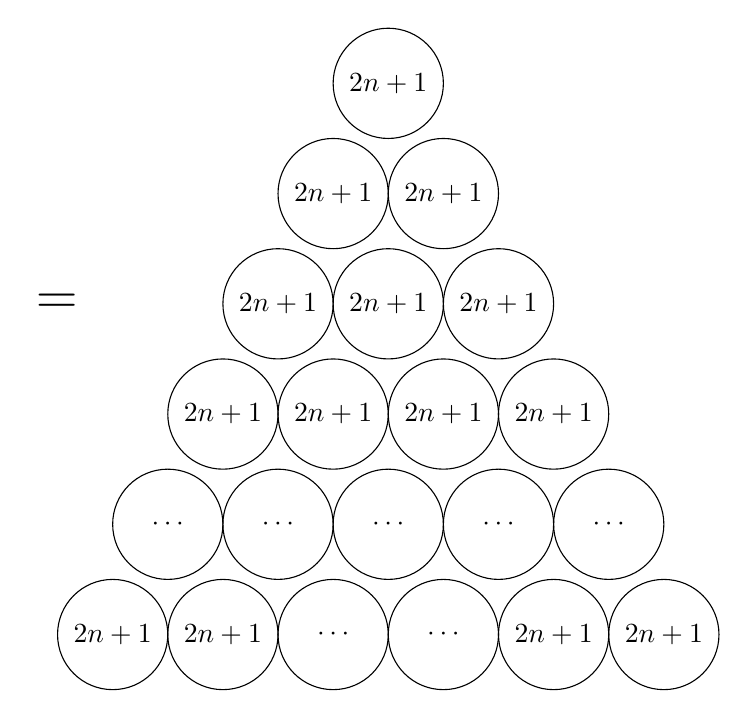
\begin{tikzpicture}[scale=1.4]
    \node at (-3,-2) {{\huge $=$}};
    \begin{scope}[shift={(0,0)}]
      \fixedcirclenode{(0,0)}{.5}{$2n+1$};
      \fixedcirclenode{(-.5,-1)}{.5}{$2n+1$}; \fixedcirclenode{(.5,-1)}{.5}{$2n+1$};
      \fixedcirclenode{(-1,-2)}{.5}{$2n+1$};  \fixedcirclenode{(0,-2)}{.5}{$2n+1$};  \fixedcirclenode{(1,-2)}{.5}{$2n+1$}; 
      \fixedcirclenode{(-1.5,-3)}{.5}{$2n+1$};  \fixedcirclenode{(-.5,-3)}{.5}{$2n+1$};  \fixedcirclenode{(.5,-3)}{.5}{$2n+1$}; \fixedcirclenode{(1.5,-3)}{.5}{$2n+1$}; \fixedcirclenode{(-2,-4)}{.5}{$\cdots$};
      \fixedcirclenode{(-1,-4)}{.5}{$\cdots$};  \fixedcirclenode{(0,-4)}{.5}{$\cdots$}; \fixedcirclenode{(1,-4)}{.5}{$\cdots$}; \fixedcirclenode{(2,-4)}{.5}{$\cdots$}; 
      \fixedcirclenode{(-2.5,-5)}{.5}{$2n+1$}; \fixedcirclenode{(-1.5,-5)}{.5}{$2n+1$};  \fixedcirclenode{(-.5,-5)}{.5}{$\cdots$};  \fixedcirclenode{(.5,-5)}{.5}{$\cdots$}; \fixedcirclenode{(1.5,-5)}{.5}{$2n+1$}; \fixedcirclenode{(2.5,-5)}{.5}{$2n+1$}; 
    \end{scope}
  \end{tikzpicture}
  \begin{align*}
    \text{从而有}\quad 3\left(1^2+2^2+3^2+\cdots+n^2\right) = (2n+1)\cdot \frac{n(n+1)}2
  \end{align*}
\end{example}

\pagebreak
\begin{theorem}[维维亚尼定理,Viviani's Theorem]\label{ex:vivianis-theorem}
  记等边三角形的高为$h$,三角形内任意一点$P$到三边的距离分别为$l,m,n$,则
  \begin{align}
    h=l+m+n
  \end{align}
\end{theorem}
\begin{center}
  \begin{tikzpicture}[scale=1]
    \tkzDefPoint[label=below left:$A$](0,0){A}
    \tkzDefPoint[label=below right:$B$](6,0){B}
    \tkzDefPoint[label=above:$C$](60:6){C} %polar coordinate
    \tkzDefPoint[label=below left:$P$](35:4){P}
    \coordinate(D) at ($(B)!(P)!(C)$);
    \coordinate(E) at ($(C)!(P)!(A)$);
    \coordinate(F) at ($(A)!(P)!(B)$);

    \coordinate(Q) at (0,6);
    \coordinate(C'') at ($(A)!(C)!(Q)$);
    \coordinate(P'') at ($(A)!(P)!(Q)$);
    \coordinate(MN) at($(P) + (120:6)$);
    \tkzInterLL(P,MN)(A,C)\tkzGetPoint{M};
    \tkzInterLL(P,MN)(A,B)\tkzGetPoint{N};
    \tkzInterLL(P,MN)(C,C'')\tkzGetPoint{C'};
    \tkzInterLL(P,P'')(A,C)\tkzGetPoint{P'};
    
    \coordinate(M'') at($(A)!(M)!(Q)$);

    % the altitude
    \coordinate(H) at (-1,0);
    \coordinate(H') at (-1,6);
    \coordinate(H'') at ($(H)!(C)!(H')$);
    \draw[|<->|](H)--(H'') node[midway,fill=white]{$h$};

    \tkzMarkRightAngle[color=blue](B,D,P)
    \tkzMarkRightAngle[color=blue](C,E,P)
    \tkzMarkRightAngle[color=blue](A,F,P)

    \tkzDrawPoints(A,B,C,P,D,E,F,C',C'',P',P'',M,M'',N);
    \tkzLabelPoints[above](C')

    \draw[very thick](A)--(B)--(C)--cycle;
    \draw(P)--(D) node[pos=0.45,above]{$l$}
         (P)--(E) node[pos=0.7, below]{$m$}
         (P)--(F) node[midway, left]{$n$}
         (A)--(P'') node[midway, left]{$n$}
         (P'')--(M'') node[midway,left]{$m$}
         (M'')--(C'') node[midway,left]{$l$};
    \draw[dashed](P)--(P'') (M)--(M'') (C)--(C'') (N)--(C');
    \tkzMarkRightAngle[color=blue](P,P'',A)
    \tkzMarkRightAngle[color=blue](M,M'',A)
    \tkzMarkRightAngle[color=blue](C,C'',A)
    \tkzMarkRightAngle[color=blue](Q,A,B)

    \draw[red,thick](P)--(P')--(C)--(C')--cycle;
  \end{tikzpicture}
\end{center}

\begin{center}
  \begin{tikzpicture}[scale=.7]
    \begin{scope}[shift={(0,0)}]
      \tkzDefPoint(0,0){A}
      \tkzDefPoint(6,0){B}
      \tkzDefPoint(60:6){C} %polar coordinate
      \tkzDefPoint(35:4){P}
      \coordinate(D) at ($(B)!(P)!(C)$);
      \coordinate(E) at ($(C)!(P)!(A)$);
      \coordinate(F) at ($(A)!(P)!(B)$);
      
      \coordinate(F1) at ($(P)!sqrt(4/3)!30:(F)$);
      \coordinate(F2) at ($(P)!sqrt(4/3)!-30:(F)$);

      \coordinate(E1) at ($(P)!sqrt(4/3)!30:(E)$);
      \coordinate(E2) at ($(P)!sqrt(4/3)!-30:(E)$);

      \coordinate(D1) at ($(P)!sqrt(4/3)!30:(D)$);
      \coordinate(D2) at ($(P)!sqrt(4/3)!-30:(D)$);
      
      \coordinate(O) at ($1/3*(P)+1/3*(E1)+1/3*(E2)$);
      \calcLength(O,E1){r}
      \centerarc[->](O)(75:-15:\r pt);
      \centerarc[->](O)(-45:-135:\r pt);
      \centerarc[->](O)(-165:-255:\r pt);

      \draw[fill=red!30] (P)--(F1)--(F2)--cycle;
      \draw[fill=violet!30] (P)--(D1)--(D2)--cycle;
      \draw[fill=blue!30]  (P)--(E1)--(E2)--cycle;
      \draw (A)--(B)--(C)--cycle;
      \draw[very thick] (P)--(D) (P)--(E) (P)--(F);
    \end{scope}
    \begin{scope}[shift={(6.5,3)}]
      \node at (0,0) {\huge $\implies$};
    \end{scope}
    \begin{scope}[shift={(7,0)}]
      \tkzDefPoint(0,0){A}
      \tkzDefPoint(6,0){B}
      \tkzDefPoint(60:6){C} %polar coordinate
      \tkzDefPoint(35:4){P}
      \coordinate(D) at ($(B)!(P)!(C)$);
      \coordinate(E) at ($(C)!(P)!(A)$);
      \coordinate(F) at ($(A)!(P)!(B)$);
      
      \coordinate(F1) at ($(P)!sqrt(4/3)!30:(F)$);
      \coordinate(F2) at ($(P)!sqrt(4/3)!-30:(F)$);

      \coordinate(E1) at ($(P)!sqrt(4/3)!30:(E)$);
      \coordinate(E2) at ($(P)!sqrt(4/3)!-30:(E)$);

      \coordinate(D1) at ($(P)!sqrt(4/3)!30:(D)$);
      \coordinate(D2) at ($(P)!sqrt(4/3)!-30:(D)$);

      \coordinate(E') at ($(E2)!(E1)!(P)$);
      
      \draw[fill=red!30] (P)--(F1)--(F2)--cycle;
      \draw[fill=violet!30] (P)--(D1)--(D2)--cycle;
      \draw[fill=blue!30]  (P)--(E1)--(E2)--cycle;
      \draw (A)--(B)--(C)--cycle;
      \draw[very thick] (P)--(D) (E1)--(E') (P)--(F);

      \coordinate(O) at ($1/3*(C)+1/3*(E1)+1/3*(D2)$);
      \calcLength(O,E1){r}
      \centerarc[->](O)(75:-15:\r pt);
      \centerarc[->](O)(-45:-135:\r pt);
      \centerarc[->](O)(-165:-255:\r pt);
    \end{scope}
    \begin{scope}[shift={(13.5,3)}]
      \node at (0,0) {\huge $\implies$};
    \end{scope}
    \begin{scope}[shift={(14,0)}]
      \tkzDefPoint(0,0){A}
      \tkzDefPoint(6,0){B}
      \tkzDefPoint(60:6){C} %polar coordinate
      \tkzDefPoint(35:4){P}
      \coordinate(D) at ($(B)!(P)!(C)$);
      \coordinate(E) at ($(C)!(P)!(A)$);
      \coordinate(F) at ($(A)!(P)!(B)$);
      
      \coordinate(F1) at ($(P)!sqrt(4/3)!30:(F)$);
      \coordinate(F2) at ($(P)!sqrt(4/3)!-30:(F)$);

      \coordinate(E1) at ($(P)!sqrt(4/3)!30:(E)$);
      \coordinate(E2) at ($(P)!sqrt(4/3)!-30:(E)$);

      \coordinate(D1) at ($(P)!sqrt(4/3)!30:(D)$);
      \coordinate(D2) at ($(P)!sqrt(4/3)!-30:(D)$);

      \coordinate(E') at ($(E2)!(E1)!(P)$);
      
      \draw[fill=red!30] (P)--(F1)--(F2)--cycle;
      \draw (A)--(B)--(C)--cycle;
      \draw[very thick] (P)--(F);
      \draw (C)--(E1)--(D2)--cycle;

      \coordinate(O) at ($1/3*(C)+1/3*(E1)+1/3*(D2)$);
      \coordinate(P) at ($(O)!1!-120:(P)$);
      \coordinate(D1) at ($(O)!1!-120:(D1)$);
      \coordinate(D2) at ($(O)!1!-120:(D2)$);
      \coordinate(D)  at ($(O)!1!-120:(D)$);
      \coordinate(E1) at ($(O)!1!-120:(E1)$);
      \coordinate(E2) at ($(O)!1!-120:(E2)$);
      \coordinate(E') at ($(O)!1!-120:(E')$);
      % \draw(C)--(O);
      % \begin{scope}[rotate around={-60:(O)}]
        \draw[rotate around={-120:(O)},fill=violet!30] (P)--(D1)--(D2)--cycle;
        \draw[rotate around={-120:(O)},fill=blue!30] (P)--(E1)--(E2)--cycle;
        \draw[rotate around={-120:(O)},very thick] (P)--(D) (E1)--(E');
      % \end{scope}
    \end{scope}
  \end{tikzpicture}
\end{center}

\pagebreak
\begin{example}%\mbox{}\par\nopagebreak
  \begin{align*}
    \sum\limits_{n=1}^\infty \left(\dfrac14\right)^n = \dfrac13
  \end{align*}
\centering
\begin{tikzpicture}[scale=0.2]
  \begin{scope}[shift={(0,0)}]
    % \node[left] at (-40,-16) {$\sum\limits_{n=1}^\infty \left(\dfrac14\right)^n = \dfrac13$};
    \draw(0,-1)rectangle(-1,0) rectangle(-2,-1)rectangle(-1,-2)rectangle(0,-1);
    \fill(-1,-1)rectangle(-2,-2);

    \draw[scale=2](0,-1)rectangle(-1,0) rectangle(-2,-1)rectangle(-1,-2)rectangle(0,-1);
    \fill[scale=2](-1,-1)rectangle(-2,-2);

    \draw[scale=4](0,-1)rectangle(-1,0) rectangle(-2,-1)rectangle(-1,-2)rectangle(0,-1);
    \fill[scale=4](-1,-1)rectangle(-2,-2);

    \draw[scale=8](0,-1)rectangle(-1,0) rectangle(-2,-1)rectangle(-1,-2)rectangle(0,-1);
    \fill[scale=8](-1,-1)rectangle(-2,-2);

    \draw[scale=16](0,-1)rectangle(-1,0)rectangle(-2,-1)rectangle(-1,-2)rectangle(0,-1);
    \fill[scale=16](-1,-1)rectangle(-2,-2);

    \node at(-16,-37) {每个\hskip5pt\tikz[scale=0.5]{\fill(0,0)rectangle(1,1);\draw(0,1)rectangle(1,2) (1,0)rectangle(2,1);}\hskip5pt 中阴影部分占$\dfrac13$};
  \end{scope}

  \begin{scope}[shift={(19,0)}]
    \draw(0,0)--(-1,-2)--(1,-2)--cycle;
    \fill[draw](-.5,-1)--(0,-2)--(.5,-1)--cycle;

    \draw[scale=2](0,0)--(-1,-2)--(1,-2)--cycle;
    \fill[scale=2,draw](-.5,-1)--(0,-2)--(.5,-1)--cycle;

    \draw[scale=4](0,0)--(-1,-2)--(1,-2)--cycle;
    \fill[scale=4,draw](-.5,-1)--(0,-2)--(.5,-1)--cycle;

    \draw[scale=8](0,0)--(-1,-2)--(1,-2)--cycle;
    \fill[scale=8,draw](-.5,-1)--(0,-2)--(.5,-1)--cycle;

    \draw[scale=16](0,0)--(-1,-2)--(1,-2)--cycle;
    \fill[scale=16,draw](-.5,-1)--(0,-2)--(.5,-1)--cycle;

    \node at(0,-38.1) {每个\hskip5pt\tikz[scale=0.5]{\fill(-.5,-1)--(0,-2)--(.5,-1)--cycle;\draw(-.5,-1)--(-1,-2)--(1,-2)--(.5,-1)--cycle;}\hskip5pt 中阴影部分占$\dfrac13$};
  \end{scope}
\end{tikzpicture}


\end{example}

\begin{example}\label{ex:pww-3-lt-pi-lt-4}
  证明:$3<\pi<4$。

\begin{center}
  \begin{tikzpicture}[scale=2]
    \begin{scope}[shift={(0,0)}]
      \draw(0,0)circle(1);
      \draw(0:1)\foreach \x in {60,120,...,360} {  -- (\x:1) } --cycle;
      \draw(0:1)--(180:1) (60:1)--(240:1) (120:1)--(300:1);
      \node[label=below:{比周长$6<2\pi$}] at (0,-1.3) {};
    \end{scope}
    \begin{scope}[shift={(3,0)}]
      \draw(0,0)circle(1);
      \draw(-1,-1)grid(1,1);
      \node[label=below:{比面积$\pi<4$}] at (0,-1.3) {};
    \end{scope}
  \end{tikzpicture}
\end{center}
\end{example}


\pagebreak
\begin{example}
  正方形$ABCD$和直角三角形$ABE$,则$\angle AEB$的角平分线将正方形$ABCE$分为两个全等的部分。\nopagebreak

  % \nopagebreak has no effect before a \begin{center} environment
\centering
  \begin{tikzpicture}[scale=.7,line join=round]
    \begin{scope}[shift={(0,0)}]
      \coordinate[label=left:$A$](A) at (0,0);
      \coordinate[label=above:$B$](B) at (4,2);
      \coordinate[label=right:$C$](C) at ($(B)!1!90:(A)$);
      \coordinate[label=below:$D$](D) at ($(C)!1!90:(B)$);
      \coordinate(E') at ($(B)!0.2!-50:(A)$);
      \coordinate[label=above:$E$](E) at ($(B)!(A)!(E')$);

      % middle of AB
      % \coordinate[label=above right:$F$](F) at ($(A)!.5!(B)$);
      % bisector of AEB
      \tkzDefLine[bisector](A,E,B)\tkzGetPoint{f}
      \tkzInterLL(A,B)(E,f)\tkzGetPoint{F}\tkzLabelPoints[above](F)

      \tkzInterLL(E,F)(C,D)\tkzGetPoint{G}\tkzLabelPoints[below](G)
      \tkzDrawPoints(A,B,C,D,E,F,G)

      \tkzMarkRightAngle[color=blue](B,E,A);
      \fill[pattern=horizontal lines,pattern color=red!30](A)--(F)--(G)--(D)--cycle;
      \fill[pattern=vertical lines,pattern color=blue!30](F)--(G)--(C)--(B)--cycle;
      \draw(A)--(B)--(C)--(D)--cycle;
      \draw(A)--(E)--(B) (E)--(F)--(G);
    \end{scope}

    \begin{scope}[shift={(10,0)}]
      \coordinate[label=left:$A$](A) at (0,0);
      \coordinate[label=above:$B$](B) at (4,2);
      \coordinate[label=right:$C$](C) at ($(B)!1!90:(A)$);
      \coordinate[label=below:$D$](D) at ($(C)!1!90:(B)$);
      \coordinate(E') at ($(B)!0.2!-50:(A)$);
      \coordinate[label=above:$E$](E) at ($(B)!(A)!(E')$);

      % middle of AB
      % \coordinate[label=above right:$F$](F) at ($(A)!.5!(B)$);
      % bisector of AEB
      \tkzDefLine[bisector](A,E,B)\tkzGetPoint{f}
      \tkzInterLL(A,B)(E,f)\tkzGetPoint{F}\tkzLabelPoints[above](F)

      \tkzInterLL(E,F)(C,D)\tkzGetPoint{G}\tkzLabelPoints[below](G)
      \tkzDrawPoints(A,B,C,D,E,F,G)

      \tkzMarkRightAngle[color=blue](B,E,A);
      \fill[pattern=horizontal lines,pattern color=red!30](A)--(F)--(G)--(D)--cycle;
      \fill[pattern=vertical lines,pattern color=blue!30](F)--(G)--(C)--(B)--cycle;
      \draw(A)--(B)--(C)--(D)--cycle;
      \draw(A)--(E)--(B) (E)--(F)--(G);

      \coordinate[label=left:$L$](L) at ($(E)!(D)!(A)$);
      \coordinate[label=right:$M$](M) at ($(E)!(C)!(B)$);
      \tkzInterLL(M,C)(L,D)\tkzGetPoint{N}\tkzLabelPoints[below](N)
      \draw[dashed](B)--(M)--(C)--(N)--(D)--(L)--(A) (G)--(N);
    \end{scope}
  \end{tikzpicture}
\end{example}

\pagebreak
\begin{example}
  将$x^2+ax$配方,有
  \begin{align*}
    x^2+ax=\left(x+\frac a2\right)^2-\left(\frac a2\right)^2
  \end{align*}
\end{example}\nopagebreak
\begin{center}
  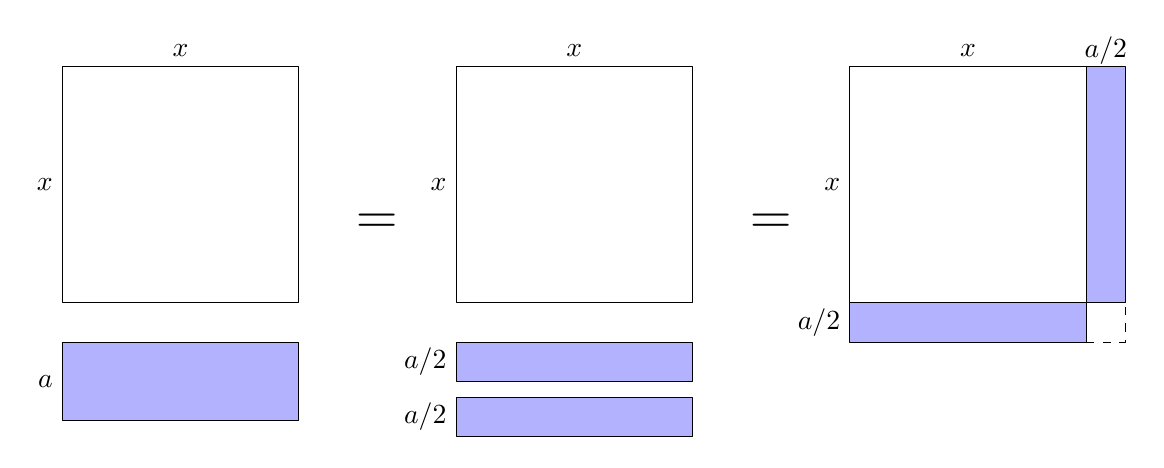
\begin{tikzpicture}[scale=1,line join=round]
    \begin{scope}[shift={(0,0)}]
      \draw (0,0)rectangle(3,3);
      \draw[fill=blue!30] (0,-.5) rectangle(3,-1.5);
      \node at (0,1.5)[left]{$x$};
      \node at (1.5,3)[above]{$x$};
      \node at (0,-1)[left]{$a$};
    \end{scope}
    
    \begin{scope}[shift={(4,0)}]
      \node at (0,1) {\huge $=$};
    \end{scope}
    
    \begin{scope}[shift={(5,0)}]
      \draw (0,0)rectangle(3,3);
      \draw[fill=blue!30] (0,-.5) rectangle(3,-1);
      \draw[fill=blue!30] (0,-1.2) rectangle(3,-1.7);
      \node at (0,1.5)[left]{$x$};
      \node at (1.5,3)[above]{$x$};
      \node at (0,-.75)[left]{$a/2$};
      \node at (0,-1.45)[left]{$a/2$};
    \end{scope}

    \begin{scope}[shift={(9,0)}]
      \node at (0,1) {\huge $=$};
    \end{scope}

    \begin{scope}[shift={(10,0)}]
      \draw (0,0)rectangle(3,3);
      \draw[fill=blue!30] (0,0) rectangle(3,-.5);
      \draw[fill=blue!30] (3,0) rectangle(3.5,3);
      \draw[dashed](3,-.5)--(3.5,-.5)--(3.5,0);
      \node at (0,1.5)[left]{$x$};
      \node at (1.5,3)[above]{$x$};
      \node at (0,-.25)[left]{$a/2$};
      \node at (3.25,2.9)[above]{$a/2$};
    \end{scope}
  \end{tikzpicture}
\end{center}

\begin{example}
  \begin{align*}
    (a+b)^2+(a-b)^2=2(a^2+b^2)
  \end{align*}
  \centering
  \begin{tikzpicture}[scale=.30]
    \begin{scope}[shift={(0,0)}]
      \draw(0,0)rectangle(8,8);
      \draw[pattern=checkerboard](6,0)rectangle(8,4) (0,6)rectangle(4,8);
      \draw[pattern=dots](6,4)rectangle(8,6) (4,6)rectangle(6,8);
      \draw[dashed](0,4)--(8,4) (4,0)--(4,8);
      \draw[|<->|](0,-1)--(6,-1)node[midway,below]{$a$};
      \draw[|<->|](6,-1)--(8,-1)node[midway,below]{$b$};
      \draw[|<->|](9,6)--(9,8)node[midway,right]{$b$};
      \draw[|<->|](9,6)--(9,4)node[midway,right]{$b$};
      \draw[|<->|](-1,0)--(-1,6)node[midway,left]{$a$};
    \end{scope}
    \node at(10,2) {\huge$+$};
    \begin{scope}[shift={(12,0)}]
      \draw[pattern=bricks](0,0)rectangle(4,4);
      \draw[|<->|](0,-1)--(4,-1)node[midway,,below]{$a-b$};
    \end{scope}
    \node at(18,2) {\huge$=$};
    \begin{scope}[shift={(20,0)}]
      \draw(0,0)rectangle(6,6)rectangle(8,8);
      \draw[|<->|](0,-1)--(6,-1)node[midway,,below]{$a$};
      \draw[|<->|](6,-1)--(8,-1)node[midway,,below]{$b$};
    \end{scope}
    \node at(29,2) {\huge$+$};
    \begin{scope}[shift={(32,0)}]
      \draw[pattern=bricks](0,0)rectangle(4,4);
      \draw[pattern=checkerboard](4,0)rectangle(6,4) (0,4)rectangle(4,6);
      \draw[pattern=dots](4,4)rectangle(6,6) rectangle(8,8);
      \draw[dashed](4,6)--(4,4)--(6,4);
      \draw[|<->|](0,-1)--(6,-1)node[midway,,below]{$a$};
      \draw[|<->|](6,-1)--(8,-1)node[midway,below]{$b$};
    \end{scope}
  \end{tikzpicture}
\end{example}

\begin{example}\mbox{}\par
  \centering
    \begin{tikzpicture}[scale=1.0]
      \node[left] at (-1.5,1.5){$(a+b+c)^2 = a^2 + b^2 + c^2 + 2ab + 2bc + 2ca$};
      \foreach \i/\x in {0/0, 1/.5, 2/1.5, 3/3}{
        \foreach \j/\y in {0/0, 1/.5, 2/1.5, 3/3}{
          \coordinate(N\i\j)at(\x,\y);
        }
      }
      \fill[color=blue!10](N00)rectangle(N11)rectangle(N22)rectangle(N33);
      \draw(N00)--(N10)node[midway,below]{$a$}
                --(N20)node[midway,below]{$b$}
                --(N30)node[midway,below]{$c$}
                --(N33)--(N03)
                --(N02)node[midway,left]{$c$}
                --(N01)node[midway,left]{$b$}
                --(N00)node[midway,left]{$a$}
           (N10)--(N13) (N20)--(N23)
           (N01)--(N31) (N02)--(N32);
      \foreach \x/\y/\t in {%
        N00/N11/$a^2$, N10/N21/$ab$, N20/N31/$ca$,
        N01/N12/$ab$, N11/N22/$b^2$, N21/N32/$bc$,
        N02/N13/$ca$, N12/N23/$bc$, N22/N33/$c^2$%
      }{
        \node at($.5*(\x)+.5*(\y)$){\t};
      }
    \end{tikzpicture}
\end{example}

\pagebreak
\begin{example}\mbox{}\par
  \centering
  \begin{tikzpicture}[scale=.5]
    \node[left] at (-3,3){$a^2 - b^2 = (a+b)(a-b)$};
    \fill[color=blue!10](4,4)rectangle(6,6);
    \fill[pattern=crosshatch, pattern color=red!20](0,4)rectangle(4,6);
    \fill[pattern=crosshatch, pattern color=red!20](6,0)rectangle(8,4);
    \draw(0,0)grid(6,6) (6,0)grid(8,4);
    \draw[|<->|](0,-.5)--(6,-.5)node[midway,below]{$a$};
    \draw[|<->|](6,-.5)--(8,-.5)node[midway,below]{$b$};
    \draw[|<->|](4,6.5)--(6,6.5)node[midway,above]{$b$};
    \draw[|<->|](-.5,0)--(-.5,6)node[midway,left]{$a$};
    \draw[|<->|](8.5,0)--(8.5,4)node[midway,right]{$a-b$};
    \draw[|<->|](8.5,4)--(8.5,6)node[midway,right]{$b$};
  \end{tikzpicture}
\end{example}

% \pagebreak
\begin{example}[半角正切公式]\mbox{}\par\nopagebreak %to mandatorily make it break line
  \centering
    \begin{tikzpicture}[scale=.9]
      \coordinate (A) at (-4,0);
      \coordinate[label=below:$O$] (O) at (0,0);
      \coordinate (B) at (4,0);
      \coordinate (C) at ($4*(.5, {sqrt(3)*.5})$);
      \coordinate (D) at ($(A)!(C)!(B)$);
      \tkzMarkRightAngle(B,C,A)\tkzMarkRightAngle(C,D,A)
      \draw(O)--(A) node[midway,below]{1};
      \draw[very thick](O)--(C) node[pos=.45,above]{1};
      \draw[very thick](C)--(D) node[pos=.6,fill=white]{$\sin\theta$};
      \draw[very thick](O)--(D) node[midway,below]{$\cos\theta$};
      \draw(D)--(B) node[midway,below]{$1-\cos\theta$};
      \draw(A)--(C)--(B);
      \draw(B)arc(0:180:4);
      \draw pic["$\theta$",<->,draw=orange,angle eccentricity=1.6,angle radius=.6cm]{angle=D--O--C};
      \draw pic["$\frac\theta2$",<->,draw=orange,angle eccentricity=1.8,angle radius=.7cm]{angle=O--A--C};
      \draw pic["$\frac\theta2$",<->,draw=orange,angle eccentricity=1.6,angle radius=.7cm]{angle=D--C--B};
      % \draw (C)--(A)--(B)--cycle--(D);
      \node[left] at (-4,2){$\tan\dfrac\theta2=\dfrac{\sin\theta}{1+\cos\theta}=\dfrac{1-\cos\theta}{\sin\theta}$};
      \tkzDrawPoint(O)
    \end{tikzpicture}
\end{example}

\pagebreak
\begin{example}[反正切求和]\mbox{}\par\nopagebreak
\centering
  \begin{tikzpicture}[scale=0.7]
    \node[left] at (-2,3) {$\atan\dfrac12+\atan\dfrac13=\dfrac\pi4$};
    \coordinate (A) at (0,3);
    \coordinate (B) at (6,0);
    \coordinate (C) at (9,6);
    \coordinate (D) at (6,3);
    \coordinate (E) at (9,3);
    \draw[help lines,dashed](0,0)grid[step=3](9,6);
    \draw[very thick, line join=round](A)--(B)node[midway,sloped]{||}--(C)node[midway,sloped]{||}--cycle;
    \draw(A)--(E)--(C) (D)--(B);
    \draw pic["$\atan\frac12$",<->,draw=orange,angle eccentricity=2,angle radius=1.5cm]{angle=B--A--D};
    \draw pic["$\atan\frac13$",<->,draw=orange,angle eccentricity=2,angle radius=1.5cm]{angle=D--A--C};
    \tkzMarkRightAngle(A,B,C);
  \end{tikzpicture}

  \vspace*{2cm}

  \begin{tikzpicture}[scale=0.7]
    \node[left] at (-2,3.5) {$\atan\dfrac ab+\atan\dfrac{b-a}{b+a}=\dfrac\pi4$};
    \draw[help lines,dashed](0,0)grid(7,7);
    \draw (2,0) node (A){} --(7,2) node (B){} --(5,7) node (C){} --(0,5)node (D){}--cycle;
    \draw (B)--(D);
    \draw (0,5)--(0,2)--(7,2) (2,2) node (E){} --(2,0);
    \draw pic["$\atan\frac ab$",<->,draw=orange,angle eccentricity=2.8,angle radius=.8cm]{angle=E--B--A};
    \draw pic["$\atan\frac {b-a}{b+a}$",<->,draw=orange,angle eccentricity=3.8,angle radius=.6cm]{angle=D--B--E};
    \draw[|<->|] (0,-.5)--(2,-.5)node[midway,fill=white]{$a$};
    \draw[|<->|] (2,-.5)--(7,-.5)node[midway,fill=white]{$b$};
    \draw[|<->|] (7.5,0)--(7.5,2)node[midway,fill=white,sloped]{$a$};
    \draw[|<->|] (-.5,2)--(-.5,5)node[midway,fill=white,sloped]{$b-a$};
  \end{tikzpicture}

  \vspace*{2cm}

  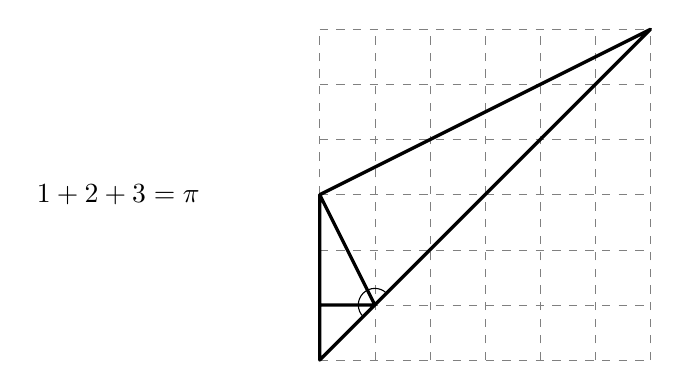
\begin{tikzpicture}[scale=0.7]
    \node[left] at(-2,3) {$\atan1+\atan2+\atan3=\pi$};
    \draw[help lines,dashed](0,0)grid(6,6);
    \draw[very thick, line join=round](0,1)--(1,1)--(0,0)--(0,3)--(1,1)--(6,6)--(0,3);
    % use coordinate transform to draw the arc: ([shift=(t:r)] x, y),
    % where (x,y) is the center and (t:r) is the polar coordinate of
    % starting point.
    \draw([shift=(225:0.3)] 1,1) arc(225:45:0.3);
  \end{tikzpicture}
\end{example}


\section{几何}
\label{sec:proofs-without-words-geometry}

\begin{example}[American Mathematical Monthly 1989]
  考虑由一个个小三角形组成的正六边形棋盘,现在请你用右边的三种(仅朝向不同的)菱形把整个棋盘全部摆满(图中只摆了其中一部分),证明当你摆满整个棋盘后,你所使用的每种菱形数量一定相同。
  \begin{center}
    \begin{tikzpicture}[scale=.5]
      \begin{scope}
        \coordinate(O)at(0,0);
        \foreach \x in{1,2,3,4,5,6}{
          \coordinate(N\x)at(60*\x-30:4);
        }
        \draw[very thick](N1)--(N2)--(N3)--(N4)--(N5)--(N6)--cycle
                         ($.5*(N2)+.5*(N3)$)--++(-30:1)
                                            --++(-90:1)
                                            --++(30:2)
                                            --++(90:1)
                                            --++(210:1)
                                            --++(210:1)
                         ($.75*(N2)+.25*(N3)$)--++(-30:1)
                                              --++(-90:1)
                                              --++(-30:1)
                                              --++( 30:1)
                                              --++(150:1)
                         ($.5*(N2)+.5*(N1)$)--++(-90:1);
        \foreach \a/\b/\c/\d in{N1/N6/N2/N3, N1/N2/N4/N3, N2/N3/N5/N4,
          N3/N4/N6/N5, N4/N5/N1/N6, N5/N6/N2/N1%
        }{
          \foreach \x/\y in {.25/.75, .5/.5, .75/.25}{
            \draw[dashed]($\x*(\b)+\y*(\a)$)--($\x*(\d)+\y*(\c)$);
          }
        }
        \draw[dashed](N1)--(N4) (N2)--(N5) (N3)--(N6);
      \end{scope}
      \begin{scope}[shift={(6,2)}]
        \begin{scope}[shift={(0,0)}]
          \draw[very thick](0,0)--(30:1)--(0,1)--(150:1)--cycle;
          \draw[dashed](0,0)--(0,1);
        \end{scope}
        \begin{scope}[shift={(.25,-1.75)},rotate=60]
          \draw[very thick](0,0)--(30:1)--(0,1)--(150:1)--cycle;
          \draw[dashed](0,0)--(0,1);
        \end{scope}
        \begin{scope}[shift={(-.5,-4)},rotate=-60]
          \draw[very thick](0,0)--(30:1)--(0,1)--(150:1)--cycle;
          \draw[dashed](0,0)--(0,1);
        \end{scope}
      \end{scope}
      \begin{scope}[shift={(12,0)}]
        \coordinate(O)at(0,0);
        \foreach \x in{1,2,3,4,5,6}{
          \coordinate(N\x)at(60*\x-30:4);
        }
        \fill[color=blue!50](N5)--++(30:3)--++(150:1)--++(210:1)--++(150:1)--++(210:1)--++(150:1)--++(210:1)--cycle
            (N2)--++(210:3)--++(-30:1)--++(30:3)--cycle
            (0,0)--++(210:2)--++(-30:1)--++(30:1)--++(-30:1)--++(30:1)--cycle
            (150:2)--++(150:1)--++(210:1)--++(-30:1)--cycle
            (0,2)--++(-30:2)--++(30:1)--++(150:2)--cycle
            ($.5*(N1)+.5*(N6)$)--++(150:1)--++(210:1)--++(-30:1)--cycle;

        \fill[color=blue!10](0,0)--(0,2)--++(-30:2)--++(0,-1)--++(-30:1)--++(0,-2)--++(150:1)--++(0,1)--++(150:2)--cycle
        (N1)--++(0,-2)--++(150:1)--++(0,1)--++(150:2)--++(0,1)--cycle
        (N4)--++(0,3)--++(-30:1)--++(0,-3)--cycle
        (0,-1)--++(0,-1)--++(-30:1)--++(0,1)--cycle
        (210:2)--++(0,-1)--++(-30:1)--++(0,1)--cycle;

        \draw[very thick](N1)--(N2)--(N3)--(N4)--(N5)--(N6)--cycle;
        \draw[very thick]($.125*(N6)+.875*(N3)$)--++(90:1)--++(-30:1)--++(30:3)
             --++(-90:1)--++(210:4)--++(150:1)--++(30:1)--++(-30:1)
             ($.5*(N2)+.5*(N3)$)--++(-30:1)--++(-90:3)--++(-30:2)--++(-90:1)--++(150:1)--++(210:1)--++(90:1)
             ($.75*(N2)+.25*(N3)$)--++(-30:1)--++(-90:3)--++(210:1)
             ($.5*(N3)+.5*(N4)$)--++(-30:1)--++(30:3)--++(-30:2)--++(90:1)--++(150:2)
             ($.25*(N3)+.75*(N4)$)--++(-30:1)--++(30:3)--++(-30:2)--++(90:1)--++(30:1)--++(90:1)--++(150:2)
             ($.5*(N2)+.5*(N1)$)--++(-90:1)--++(210:1)--++(-90:2)--++(210:2)--++(150:1)--+(90:3)--++(-90:1)--++(210:1)--++(90:3)
             ($.25*(N2)+.75*(N1)$)--++(-90:1)--++(210:1)
             ($.5*(N4)+.5*(N5)$)--++(30:1)--+(150:1)
             (0,-1)--(0,-2)
             ($.25*(N4)+.75*(N5)$)--++(30:1)--++(150:1)
             ($.75*(N5)+.25*(N6)$)--++(150:1)--++(30:1)--++(-30:1)
             ($.75*(N1)+.25*(N6)$)--++(150:1)
             ($.5*(N1)+.5*(N6)$)--++(150:1)
             ($.5*(N1)+.5*(N6)$)--++(210:1)--++(150:1)
             ($.25*(N1)+.75*(N6)$)--++(210:1)--++(150:1)--++(210:1)
             (-30:2)--++(-90:1)--++(210:1)
             (-30:3)--++(90:1)
             (-30:3)--++(-90:1)--++(150:1);

        \foreach \a/\b/\c/\d in{N1/N6/N2/N3, N1/N2/N4/N3, N2/N3/N5/N4,
          N3/N4/N6/N5, N4/N5/N1/N6, N5/N6/N2/N1%
        }{
          \foreach \x/\y in {.25/.75, .5/.5, .75/.25}{
            \draw[dashed]($\x*(\b)+\y*(\a)$)--($\x*(\d)+\y*(\c)$);
          }
        }
        \draw[dashed](N1)--(N4) (N2)--(N5) (N3)--(N6);
      \end{scope}
    \end{tikzpicture}
  \end{center}

把每种菱形涂上一种颜色,整个图形瞬间有了立体感,看上去就成了一个个立方体在墙角堆叠起来的样子。三种菱形分别是从左侧、右侧、上方观察整个立体图形能够看到的面,它们的数目显然应该相等\footnote{这并不是严格的证明,但并不影响数学家们对此方法的喜爱。}。
\end{example}
